\documentclass[11pt, a4paper]{article}
\usepackage[paper=a4paper, left=1.5cm, right=1.5cm, bottom=1.5cm, top=1.5cm]{geometry}

\usepackage[utf8]{inputenc}
\usepackage[T1]{fontenc}
\usepackage[spanish]{babel}
\usepackage[section]{placeins}
\usepackage{caratula/caratula}
\usepackage{listings}
\usepackage{algpseudocode}
\usepackage{graphicx}
\usepackage{float}
\usepackage{amsmath}
%\usepackage{adjustbox}
\usepackage{blindtext}
\usepackage{sidecap}
\usepackage{color}
\usepackage{subfigure}
\usepackage{caption}

\begin{document}

\titulo{Trabajo Práctico \#1}
\fecha{28 de Junio de 2013}
\materia{Sistemas operativos}
% \grupo{Grupo 11}
\integrante{Leandro Matayoshi}{79/11}{leandro.matayoshi@gmail.com}
\integrante{Martin Santos}{413/11}{martin.n.santos@gmail.com}
\integrante{Alexander Szyrej}{642/11}{luzbelito.as@gmail.com}

%Carátula
\maketitle
\newpage
%Indice
\tableofcontents
\newpage


\section{Introducción}
El siguiente trabajo pretende analizar los distintos algoritmos de $scheduling$ para distintos tipos de tareas. 
Para ello implementamos diferentes tareas para simular distintos tipos de ellas, sean de procesamiento intenso o interactivas, etc.
Así mismo se implementaron distintos algoritmos de $scheduling$ para evaluar su respuesta frente a diferentes lotes de tareas mencionadas anteriormente.
Para un mejor análisis, la cátedra nos facilitó un graficador que toma de entrada el output del simulador $simusched$ (también provisto por la cátedra) que utiliza los algoritmos de $scheduling$ programados por nosotros.

El trabajo fue dividido en tres partes:

\section{Parte I: Entendiendo $simusched$}
Para la primera parte implementamos la tarea \textbf{TaskConsola}, la cual simula ser una tarea interactiva.

TaskConsola recibe tres parámetros: $n$, $bmin$ y $bmax$; y debe realizar $n$ llamadas bloqueantes, cada una con un tiempo pseudoaleatorio
entre $bmin$ y $bmax$. Con el fin de generar este tiempo debimos generar un número pseudoaleatorio $random\_number$, para lo cual utilizamos las funciones rand() y srand() definidas en la stdlib. El número es generado por rand() bajo una semilla generada por srand() en función del horario en el cual corre la tarea ($\#include <sys/time.h>$). Luego, el tiempo $t$ para la i-ésima llamada bloqueante es dado por la siguiente operación: $t = bmin + (random\_number \% (bmax-bmin+1))$, para que el número pertenezca al intervalo deseado.

~

Luego implementamos el scheduler \textbf{SchedFCFS}, que utiliza el algoritmo de First-Come First-Served. Dicho de otro modo, las tareas se ejecutan por órden de llegada y hasta que finalice su ejecución. Implementamos el SchedFCFS sobre una cola de tareas en estado $ready$, donde la función LOAD se resume en simplemente encolar el pid de la tarea a cargar; la función UNBLOCK no tiene uso dado que aún si la tarea se bloquea, esta corre en el cpu hasta que finalice su espera; y la función TICK simplemente cambia de tarea cuando se la llama con motivo de exit y la tarea que corría en el cpu termina.

~

A continuación un gráfico del comportamiento del SchedFCFS con uno, dos y tres cores, sin costos de migración o cambio de contexto, para un lote de 3 tareas, dos interactivas TaskConsola y una TaskCPU de procesamiento intensivo.

\begin{figure}[H]
\centering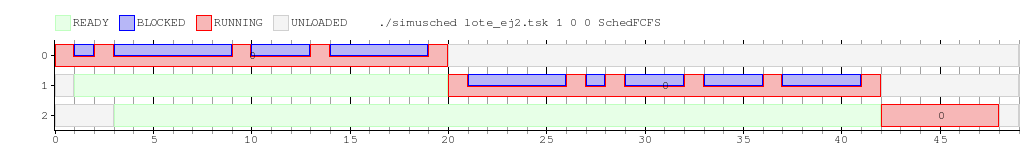
\includegraphics[width=18 cm]{graficos/ej2FCFS1.png}
\centering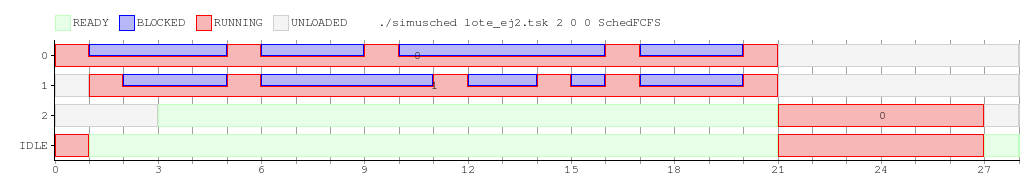
\includegraphics[width=18 cm]{graficos/ej2FCFS2.png}
\centering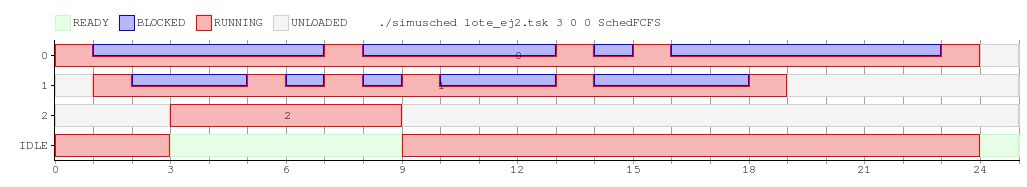
\includegraphics[width=18 cm]{graficos/ej2FCFS3.png}
\caption{First-Come First-Served, un sólo núcleo de procesamiento en el primer caso, dos en el segundo y por último tres núcleos.}
\end{figure}

Podemos ver en la figura 1 que, si bien este algoritmo evita posibles costosos cambios de contexto y costos de migración, se pierde mucha interactividad. Con un único núcleo la tarea TaskCPU debe esperar a las dos tareas bloqueantes para finalmente correr, cuando podría haber terminado si esta corría mientras las interactivas permanecían bloqueadas.

Lo mismo sucede en el segundo caso, pero desde ya al correr las TaskConsola en paralelo, esto acorta considerablemente el tiempo de espera de la tarea intensiva en CPU. Luego las tres tareas en paralelo permiten con este algoritmo ahorrar en cambios de contexto o migración, ya que otro algoritmo podrìa rotar a las tareas entre los núcleos.




\section{Parte II: Nuevos Schedulers}
Una vez que entendemos el simulador y usamos el graficador con un scheduler básico como lo es SchedFCFS nos proponemos a realizar nuevos schedulers: \textbf{SchedRR} y \textbf{SchedLottery}.

\subsection{SchedRR}

El siguiente paso fue completar la implementación de SchedRR, el cual se basa en el algoritmo de scheduling $round-robin$. 

Básicamente las tareas forman una ronda para correr en algún núcleo (de haber más de uno). Cada CPU tiene asociado un quantum máximo, es decir, una cantidad máxima de ciclos en el cual puede correr una determinada tarea. El quantum de cada CPU es parámetro de nuestro scheduler.

Así como el SchedFCFS, éste scheduler esta implementado sobre una cola de tareas global (para permitir migración), pero a diferencia del anterior, nuestro scheduler irá encolando a las tareas nuevamente en la cola una vez que sean desalojadas del CPU, ya sea por realizar una llamada bloqueante o debido a que su quantum se completó. Si la tarea se bloqueo, no sera encolada en la cola de tareas $ready$ hasta que se desbloquee, por lo cual la función UNBLOCK comienza a tener sentido y es ahi donde la tarea regresa a la cola.

Para determinar si una tarea cumplió con el quantum máximo del CPU en la cual corre tenemos un vector de quantums parciales, un contador para cada CPU. Por cada tick se incrementa en uno y se resetea en caso de que la tarea sea desalojada. Notar que si la tarea se bloquea es desalojada y por lo tanto pierde su quantum.

Como detalle de implementación determinamos que si existe una única tarea y ésta se bloquea seguirá corriendo en el CPU para evitar pagar costos de cambio de contexto.

Veamos el gráfico a continuación:

\begin{figure}[H]
\centering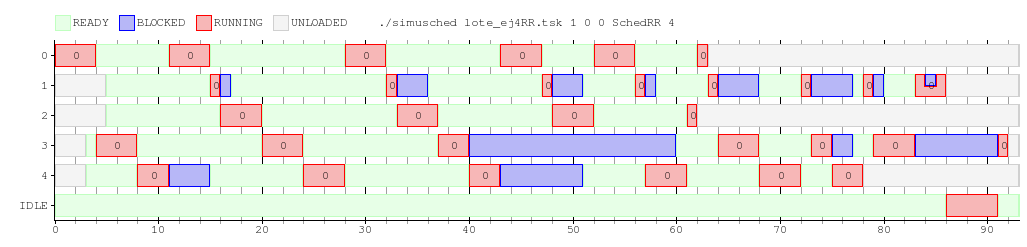
\includegraphics[width=18 cm]{graficos/ej4RR1.png}
\centering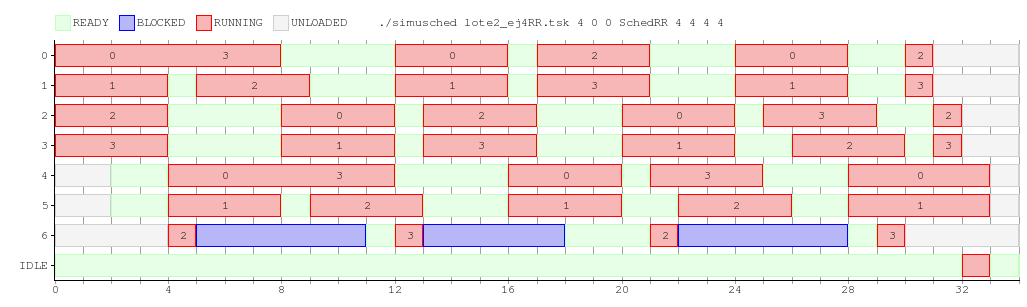
\includegraphics[width=18 cm]{graficos/ej4RR2.png}
\caption{First-Come First-Served, un sólo núcleo de procesamiento en el primer caso, dos en el segundo y por último tres núcleos.}
\end{figure}



\subsection{SchedLottery y compensaciones probabilísticas}

\subsubsection{Ecuanimidad del SchedLottery}

En el ejercicio 5 implementamos un scheduler en base al paper ''Lottery scheduling''. Intentamos generar un mecanismo de control eficiente, flexible y justo en donde cada tarea fuese procesada
aproximadamente un tiempo equivalente a las otras, sin importar su tipo. Este último aspecto es el que nos permite hablar de ecuanimidad del scheduler.

Para ejemplificar lo mencionado anteriormente, supongamos que en una computadora de un solo core se han lanzado dos procesos que corren en simultáneo. El primero de ellos, al cual llamaremos $A$, utiliza
activamente el CPU sin necesidad de hacer llamados al sistema o esperar que se liberen recursos de la máquina (podría ser, por ejemplo, el caso de una aplicación científica que ejecuta gran cantidad de 
cuentas). Por otro lado tenemos a la tarea $B$, que ejecuta una instrucción bloqueante cada cierto tiempo, desbloquéandose luego de una cierta cantidad de ticks del reloj. Supongamos también que ambos conviven
con otros procesos que también están siendo ejecutados por el cpu. En el caso de un scheduler Round Robin, a lo largo de una ronda se le asigna un quantum a cada proceso. Sin embargo, notemos que mientras
la tarea $A$ utiliza la totalidad del quantum que le han asignado, $B$ usa únicamente una fracción: $\frac{f}{q}$. De esta manera, luego de sucesivas rondas la tarea $A$ ha sido ejecutada un tiempo
considerablemente mayor al de $B$.

Para solucionar este problema, la idea es que el scheduler seleccione la próxima a ser ejecutada mediante el sorteo de una lotería, en donde aquellas tareas que utilicen solamente una fracción del quantum
tengan más probabilidades de ser las ganadoras. Para lograr este objetivo, utilizamos un sistema de ''compensation tickets'', que funciona de la siguiente manera:

- Las tareas que llegan por primera vez entran con una cantidad equivalente a $\frac{tickets}{1 \ quantum}$. Por ejemplo, si el 
- Las tareas que utilizaron la totalidad del quantum la último





 


\section{Parte III: Experimentación}
Para experimentar con los distintos algoritmos de scheduling planteados a lo largo del trabajo confeccionamos una nueva tarea 
\textbf{TaskBatch} y un "nuevo" scheduler \textbf{SchedRR2}, el cual se basa también en el algoritmo $round-robin$ pero no permite migración entre núcleos.

TaskBatch es una tarea que toma dos parámetros, $total_cpu$ y $cant_bloqueos$. Su función es bloquearse tantas veces como $cant_bloqueos$ en momentos pseudoaleatorios, pero sin excederse jamas de $total_cpu$ tiempo corriendo en el CPU. Es decir, la tarea correrá siempre un tiempo constante en el CPU, pero su tiempo total de ejecución dependerá de cuanto tiempo se bloquee y cuanto tiempo esperé en estado $ready$ para correr.

Básicamente su implementación se resume en un ciclo. Por cada iteración se genera un número pseudoaleatorio en un rango razonable, el cual se compara con ciertos parámetros para determinar, con cierta probabilidad, si se bloquea o no en ese momento. Si se bloquea, disminuimos la cantidad de bloqueos restantes. En otro caso, diminuimos el tiempo que nos queda restante (en el cual se toma en cuenta el tiempo consumido por las llamadas bloqueantes y el exit). Si vemos que el tiempo corre y faltan llamadas bloqueantes, ellas se daran al hilo al final. De otro modo, si resulta que ya se ha bloquedo las veces que queriamos, usaremos el CPU el tiempo restante.

Esa constancia en tiempo $running$ nos permite experimentar con más tranquilidad.

~

Luego nos planteamos determinar cual es el valor óptimo de quantum para ciertos schedulers, en particular experimentamos en el ejercicio 7 con el SchedRR, con costo de cambio de contexto de un ciclo y dos ciclos de costo de migración. Para ello planteamos dos diferentes métricas: TurnAround time y Waiting time.

\subsection{TurnAround time}

Aquí queremos ver como afecta el quantum que el scheduler determina para cada CPU en el tiempo de ejecución de cada tarea. Planteamos la siguiente ecuación:
\centering $\frac{\#ciclosDeEjecucion}{quantum} * (quantum + costoContexto + constoMigracion) = tiempoDeEjec$



\subsection{Waiting time}

\subsection{Quantum óptimo del SchedRR}

Para determinar el $quantum$ óptimo del scheduler $Round$ $Robin$ simulamos un lote de tareas $TaskBach$ utilizando el algoritmo SchedRR teniendo en cuenta las métricas mencionadas anteriormente: waiting time y turnaround time. Diseñamos el lote de la siguiente manera:
\begin{itemize}
	\item Cantidad de tareas: 30. Nos pareció un número adecuado para llevar a cabo el experimento.
	\item Uso de Cpu: igual para todas, 30.
	\item Cantidad de bloqueos: variados, entre 1 y 30.
\end{itemize}
(El lote de tareas utilizado puede encontrarse en el archivo $loteBatch.tsk$.)

Los costos de cambio de contexto y migración se fijaron en 1 y 2 (ciclos) respectivamente. Experimentamos utilizando varios núcleos de procesamiento.
Graficamos los resultados de waiting time y turnaround time en función del quantum para 2,3 y 4 cores. Debido a que las tareas $TaskBatch$ realizan bloqueos en momentos elegidos pseudoaleatoriamente nos pareció correcto que, para un quantum dado, se hagan varias corridas (veinte) con el fin de obtener un waiting time y turnaround time promedio. A su vez, tuvimos en cuenta el desvío estandar de estas mediciones para realizar las barras de error en los gráficos. Los resultados obtenidos fueron los siguientes:

\begin{figure}[H]
	\begin{center}
		  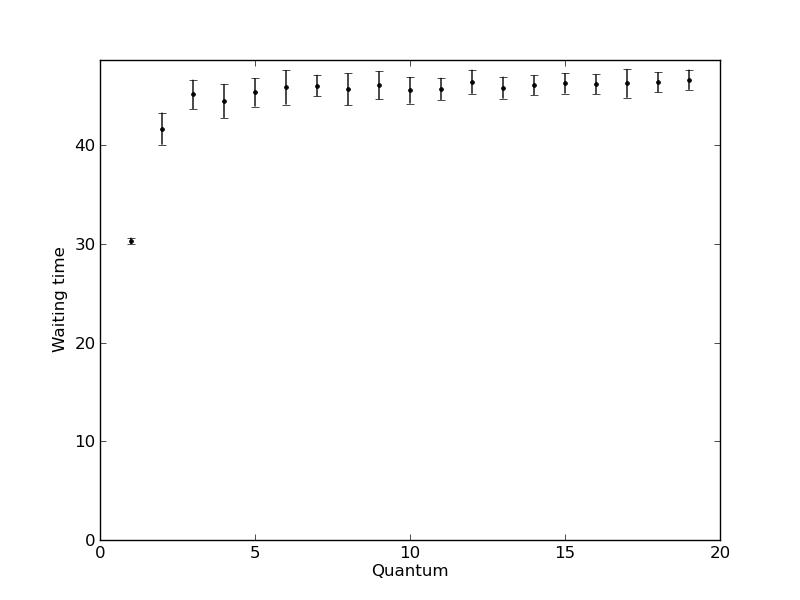
\includegraphics[scale=0.3]{graficos/cores_2_wt.jpg}
		  \caption{Representación de Waiting time en función del quantum para un procesador de 2 núcleos utilizando un lote de tareas $taskBatch$}
		  \label{fig:contra1}
	\end{center}
\end{figure}

\begin{figure}[H]
	\begin{center}
		  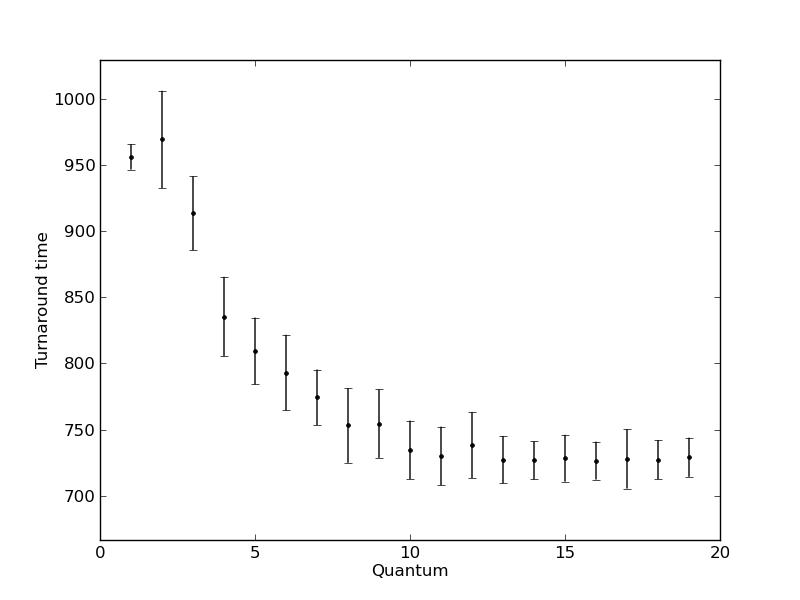
\includegraphics[scale=0.3]{graficos/cores_2_ta.jpg}
		  \caption{Representación de Turnaround time en función del quantum para un procesador de 2 núcleos utilizando un lote de tareas $taskBatch$}
		  \label{fig:contra1}
	\end{center}
\end{figure}

\begin{figure}[H]
	\begin{center}
		  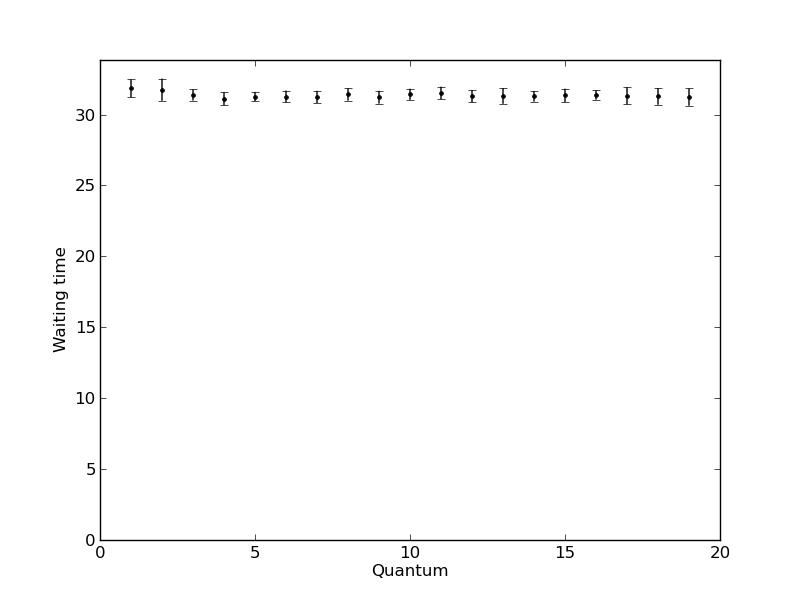
\includegraphics[scale=0.3]{graficos/cores_3_wt.jpg}
		  \caption{Representación de Waiting time en función del quantum para un procesador de 3 núcleos utilizando un lote de tareas $taskBatch$}
		  \label{fig:contra1}
	\end{center}
\end{figure}

\begin{figure}[H]
	\begin{center}
		  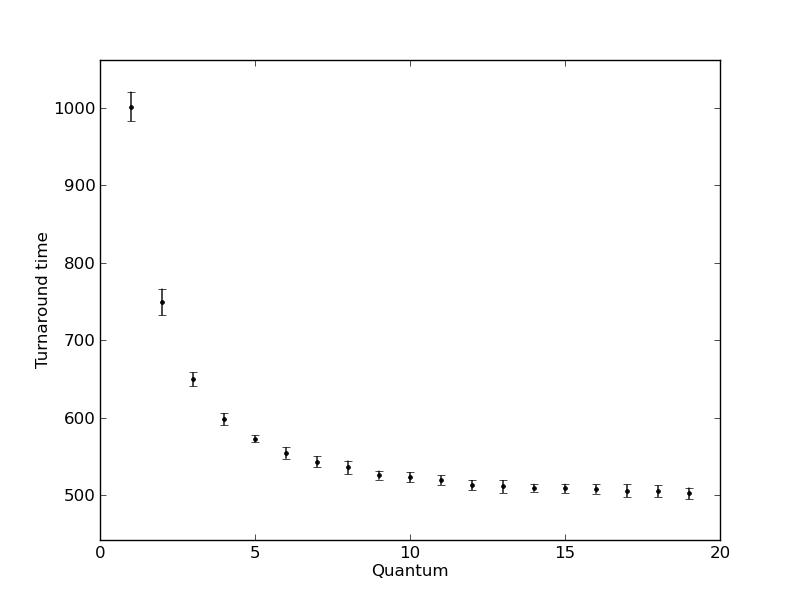
\includegraphics[scale=0.3]{graficos/cores_3_ta.jpg}
		  \caption{Representación de Turnaround time en función del quantum para un procesador de 3 núcleos utilizando un lote de tareas $taskBatch$}
		  \label{fig:contra1}
	\end{center}
\end{figure}

\begin{figure}[H]
	\begin{center}
		  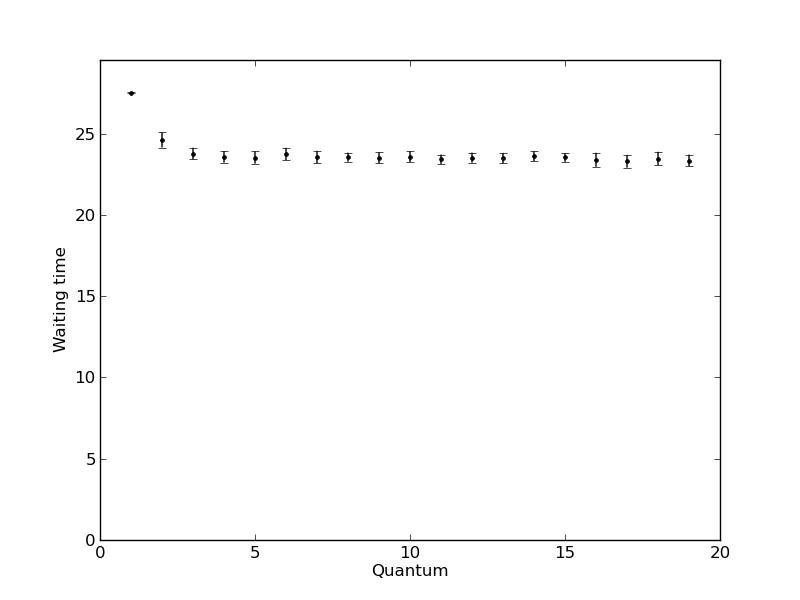
\includegraphics[scale=0.3]{graficos/cores_4_wt.jpg}
		  \caption{Representación de Waiting time en función del quantum para un procesador de 4 núcleos utilizando un lote de tareas $taskBatch$}
		  \label{fig:contra1}
	\end{center}
\end{figure}

\begin{figure}[H]
	\begin{center}
		  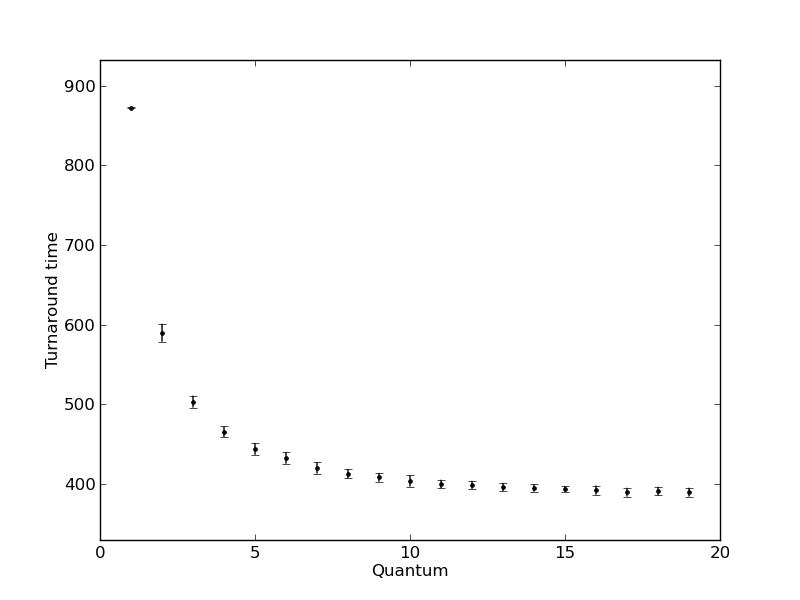
\includegraphics[scale=0.3]{graficos/cores_4_ta.jpg}
		  \caption{Representación de Turnaround time en función del quantum para un procesador de 4 núcleos utilizando un lote de tareas $taskBatch$}
		  \label{fig:contra1}
	\end{center}
\end{figure}

Como puede observarse en las figuras 8, 10 y 12, los valores de waiting time obtenidos no difieren demasiado al ir variando los quantums para cada tarea. Este comportamiento no ocurre en los gráficos de turnaround time en donde comienzan a tenerse resultados similares a partir de un quantum igual a 8. Es por esta razón que nos pareció apropiado determinar un quantum óptimo de 8 ticks para el lote de tareas $TaskBatch$ presentado.

%En los gráficos de waiting time (8, 10 y 12) podemos observar que, para cualquier quantum dado, los valores de waiting time obtenidos

%Teniendo en cuenta los gráficos 8, 10 y 12 podemos observar que los valores de waiting time obtenidos para cada quantum no difieren demasiado. Esto no ocurre para los demás graficos en donde el turnaround time comienza a estabilizarse a partir de un quantum igual a 7. Es por esta razón que nos pareció apropiado determinar un quantum óptimo de 7 ticks para el lote de tareas $TaskBatch$ presentado.


\subsection{SchedRR vs SchedRR2}

Para comparar el funcionamiento de los dos schedulers simularemos el comportamiento de ambos algoritmos utilizando tres lote de tareas:
\begin{itemize}
	\item Lote 1: combina varias tareas de uso intensivo de CPU y tareas interactivas (bloqueantes). La idea es simular un lote que podría estar corriendo en cualquier computadora hogareña. Este lote tendrá 180 tareas que es la cantidad de procesos corriendo actualmente en esta computadora.
	\item Lote 2: conformada por tareas de tipo interactivas. Simulará a un lote de tareas de un celular.
	\item Lote 3: conformada por tareas que solo hacen uso intensivo de CPU.
\end{itemize}
Para cada uno de los lotes calcularemos el waiting time y turnaround time promedio para cada scheduler tomando distintos valores de quantum y probando con 2, 3 y 4 cores. Los costos de cambio de contexto y migración serán 1 y 2 repectivamente. Teniendo en cuenta los resultados concluiremos cuál de los dos algoritmos se comporta mejor.

\subsubsection{Lote 1: Pc}

\begin{figure}[H]
\hfill
\subfigure[]{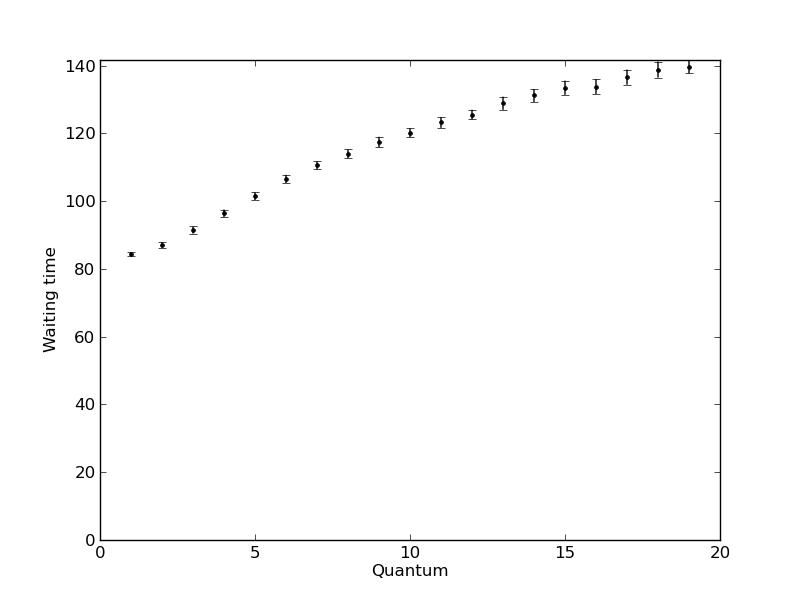
\includegraphics[width=8.75cm]{graficos/schedRR_pc/cores_2_wt.jpg}}
\hfill
\subfigure[]{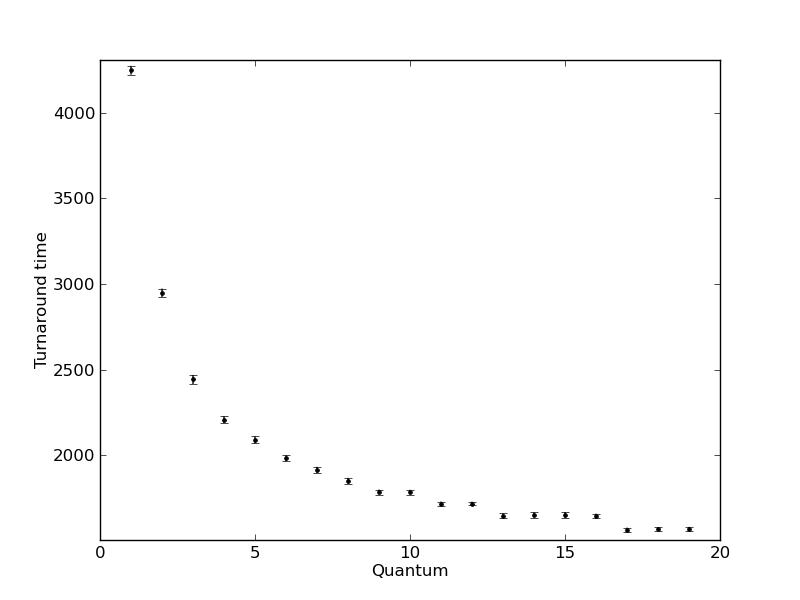
\includegraphics[width=8.75cm]{graficos/schedRR_pc/cores_2_ta.jpg}}
\hfill
\caption{Gráfico de Waiting time y turnaround time en función del quantum con 2 cores para lote de tareas $lotePc$ en SchedRR}
\end{figure}

\begin{figure}[H]
\hfill
\subfigure[]{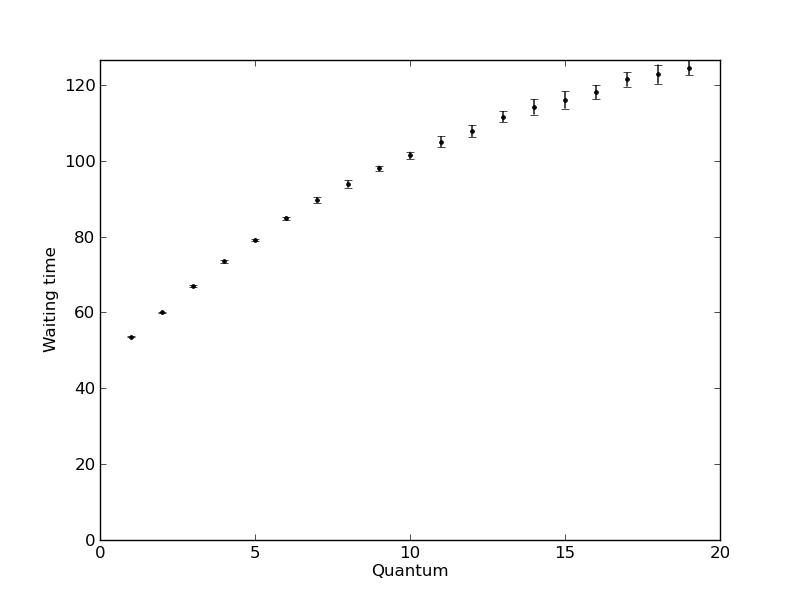
\includegraphics[width=8.75cm]{graficos/schedRR2_pc/cores_2_wt.jpg}}
\hfill
\subfigure[]{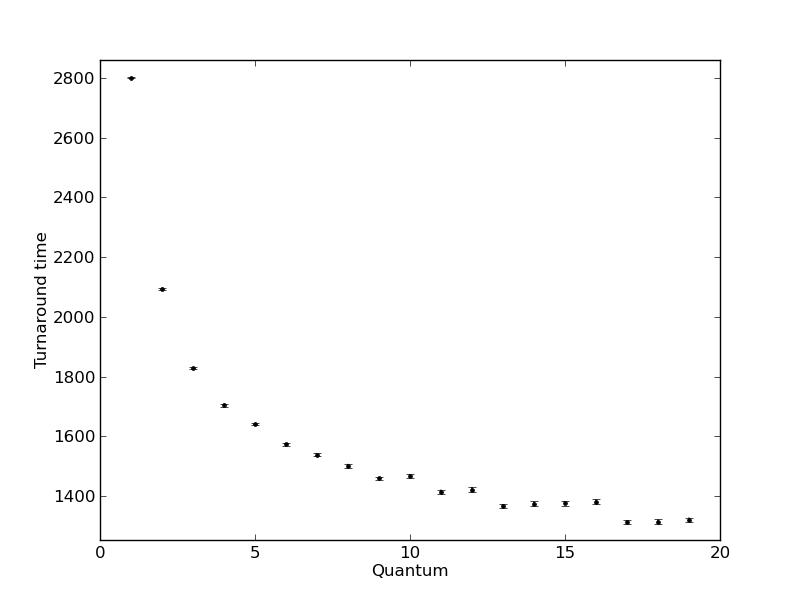
\includegraphics[width=8.75cm]{graficos/schedRR2_pc/cores_2_ta.jpg}}
\hfill
\caption{Gráfico de Waiting time y turnaround time en función del quantum con 2 cores para lote de tareas $lotePc$ en SchedRR2}
\end{figure}

\begin{figure}[H]
\hfill
\subfigure[]{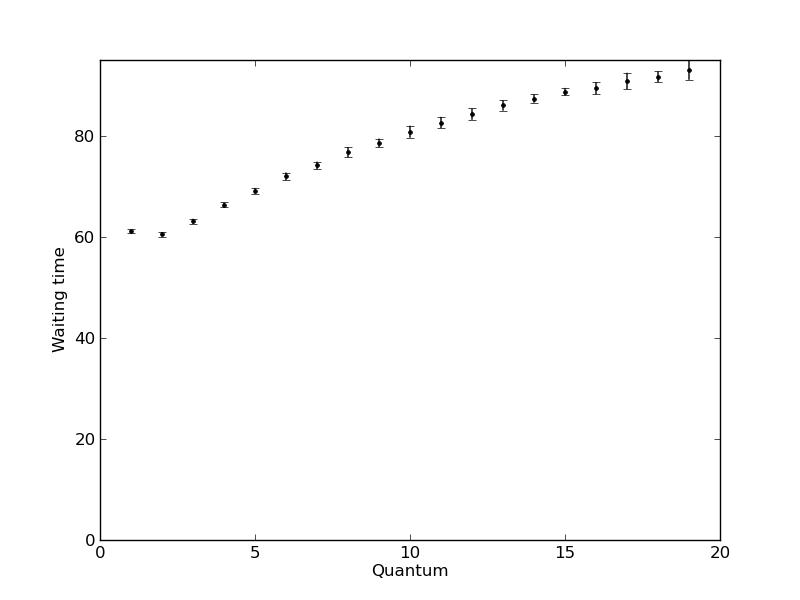
\includegraphics[width=8.75cm]{graficos/schedRR_pc/cores_3_wt.jpg}}
\hfill
\subfigure[]{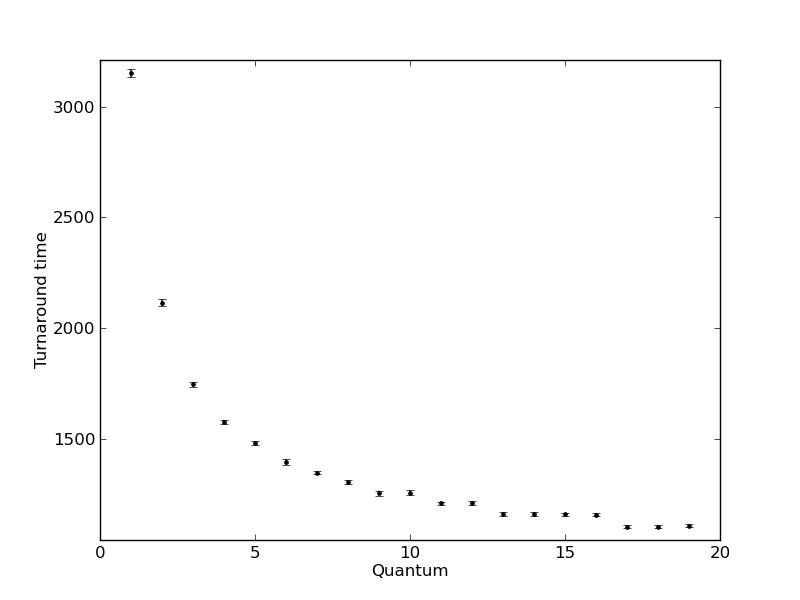
\includegraphics[width=8.75cm]{graficos/schedRR_pc/cores_3_ta.jpg}}
\hfill
\caption{Gráfico de Waiting time y turnaround time en función del quantum con 3 cores para lote de tareas $lotePc$ en SchedRR}
\end{figure}

\begin{figure}[H]
\hfill
\subfigure[]{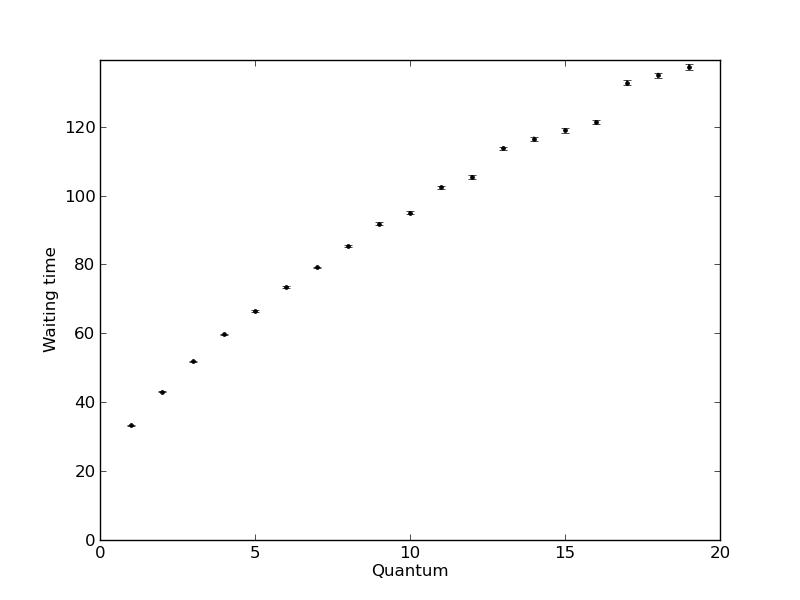
\includegraphics[width=8.75cm]{graficos/schedRR2_pc/cores_3_wt.jpg}}
\hfill
\subfigure[]{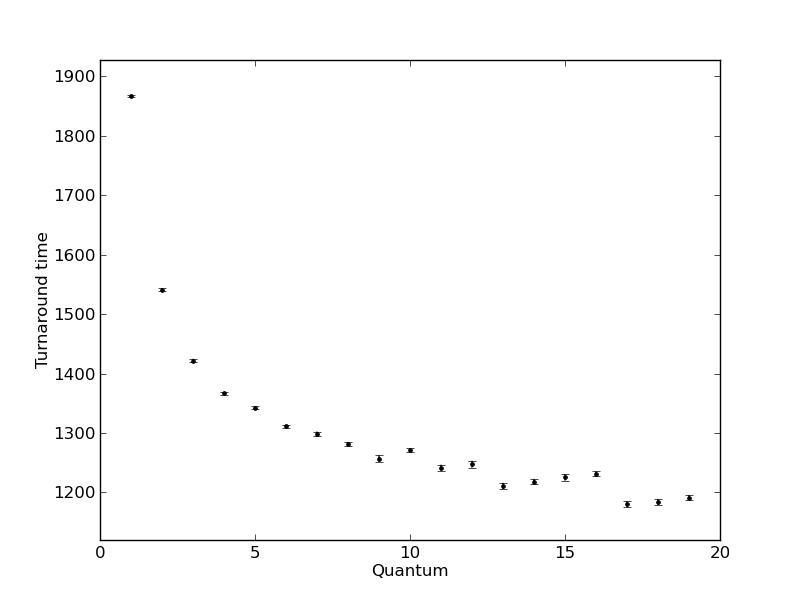
\includegraphics[width=8.75cm]{graficos/schedRR2_pc/cores_3_ta.jpg}}
\hfill
\caption{Gráfico de Waiting time y turnaround time en función del quantum con 3 cores para lote de tareas $lotePc$ en SchedRR2}
\end{figure}

\begin{figure}[H]
\hfill
\subfigure[]{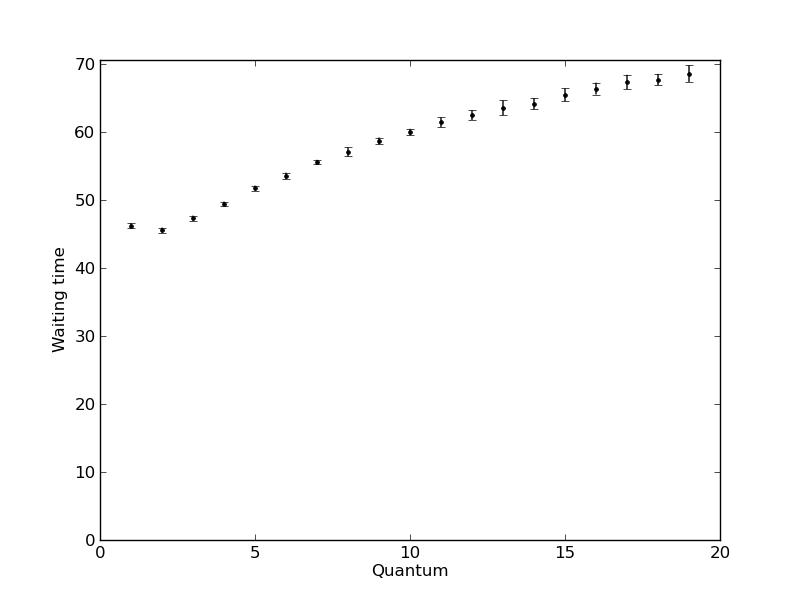
\includegraphics[width=8.75cm]{graficos/schedRR_pc/cores_4_wt.jpg}}
\hfill
\subfigure[]{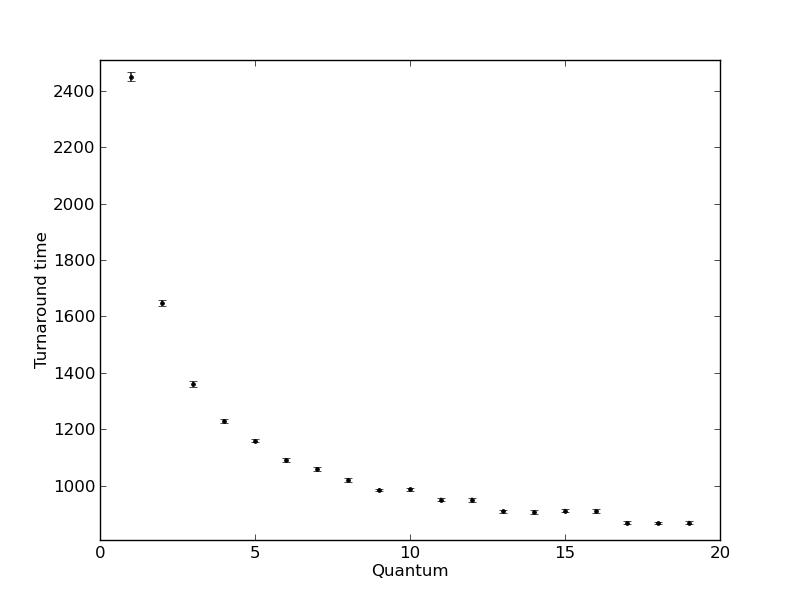
\includegraphics[width=8.75cm]{graficos/schedRR_pc/cores_4_ta.jpg}}
\hfill
\caption{Gráfico de Waiting time y turnaround time en función del quantum con 4 cores para lote de tareas $lotePc$ en SchedRR}
\end{figure}

\begin{figure}[H]
\hfill
\subfigure[]{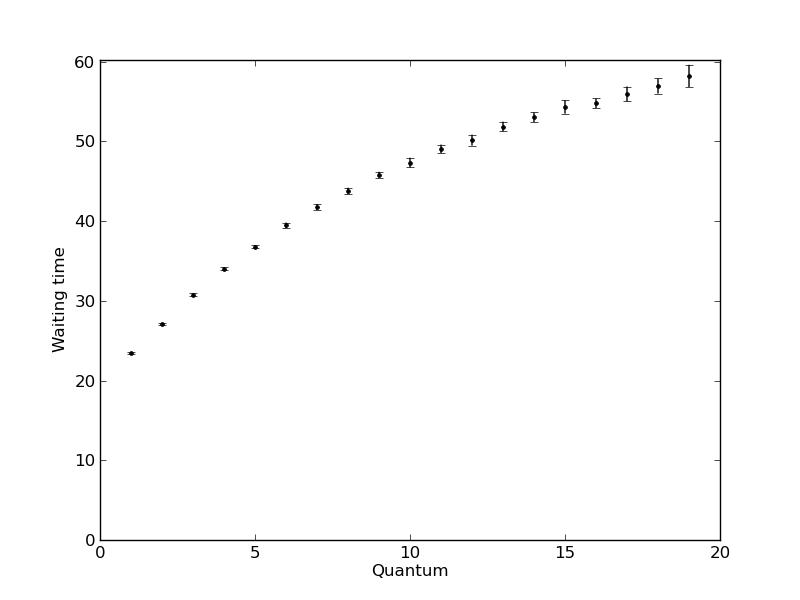
\includegraphics[width=8.75cm]{graficos/schedRR2_pc/cores_4_wt.jpg}}
\hfill
\subfigure[]{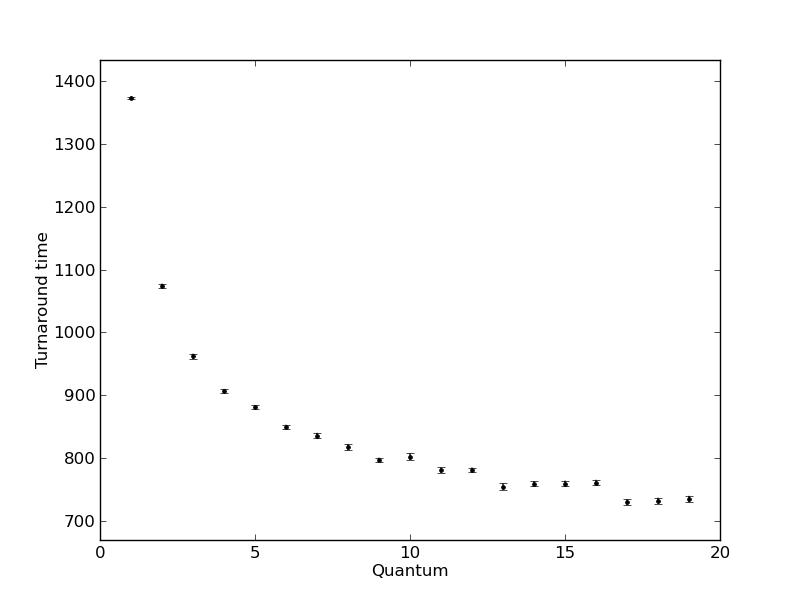
\includegraphics[width=8.75cm]{graficos/schedRR2_pc/cores_4_ta.jpg}}
\hfill
\caption{Gráfico de Waiting time y turnaround time en función del quantum con 4 cores para lote de tareas $lotePc$ en SchedRR2}
\end{figure}

\begin{center}
    \begin{tabular}{ | l | l | l | l | l | p{5cm} |}
    \hline
    Cores & Wt RR & Wt RR2 & Ta RR & Ta RR2 \\ \hline
    2 & 116.89 & 97 & 1998.06 & 1573.38 \\ \hline
    3 & 78.71 & 92.74 & 1420.25 & 1310.04 \\ \hline
    4 & 58.5 & 44.98 & 1112.45 & 847.02 \\
	\hline
    \end{tabular}
\end{center}

Observando la tabla podemos concluir que el schedRR2 tiene un mejor wt y ta en promedio para un lote de tareas pc.

\subsubsection{Lote 2: celular}

\begin{figure}[H]
\hfill
\subfigure[]{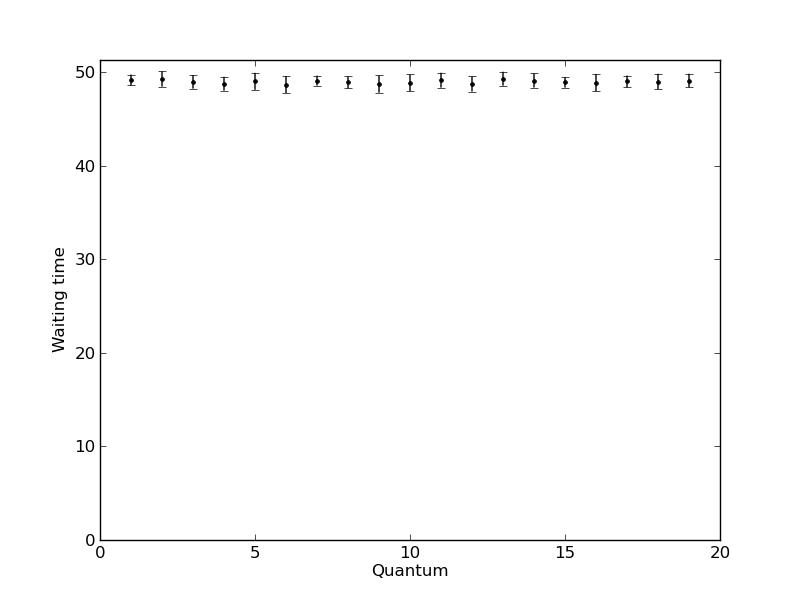
\includegraphics[width=8.75cm]{graficos/schedRR_celular/cores_2_wt.jpg}}
\hfill
\subfigure[]{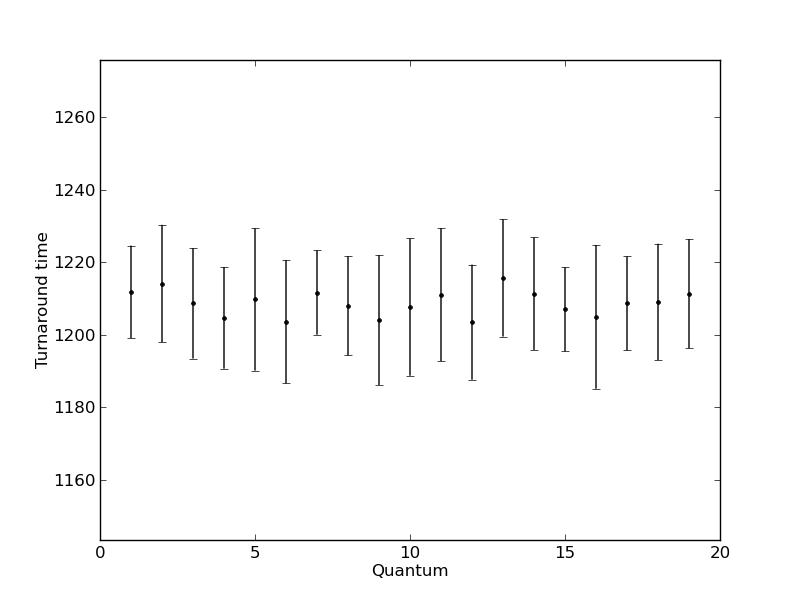
\includegraphics[width=8.75cm]{graficos/schedRR_celular/cores_2_ta.jpg}}
\hfill
\caption{Gráfico de Waiting time y turnaround time en función del quantum con 2 cores para lote de tareas $loteCelular$ en SchedRR}
\end{figure}

\begin{figure}[H]
\hfill
\subfigure[]{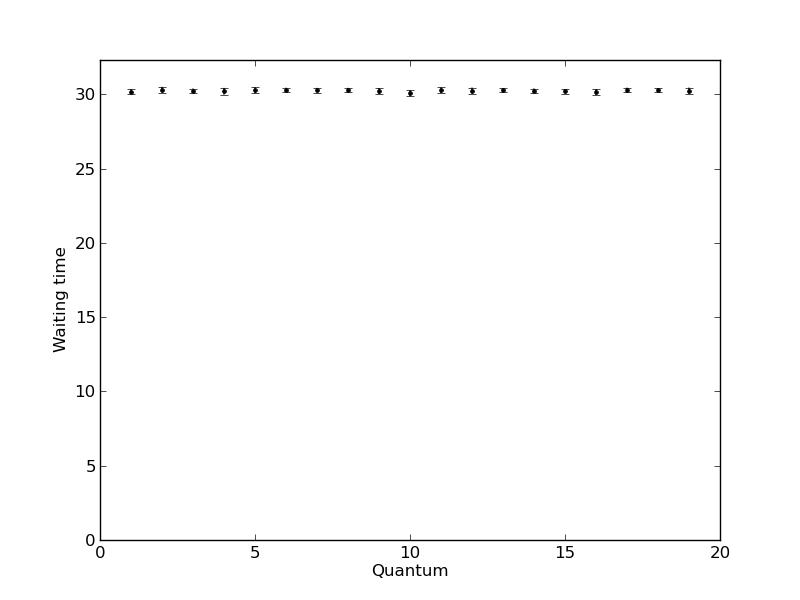
\includegraphics[width=8.75cm]{graficos/schedRR2_celular/cores_2_wt.jpg}}
\hfill
\subfigure[]{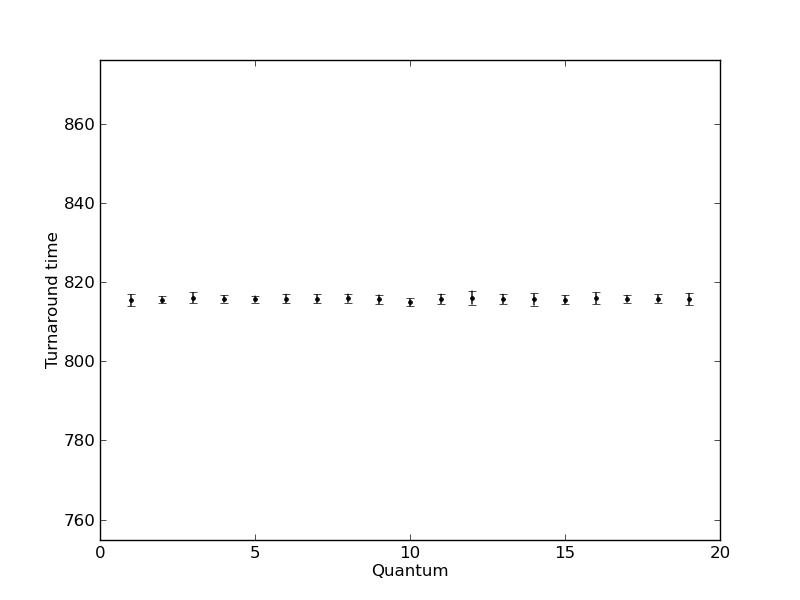
\includegraphics[width=8.75cm]{graficos/schedRR2_celular/cores_2_ta.jpg}}
\hfill
\caption{Gráfico de Waiting time y turnaround time en función del quantum con 2 cores para lote de tareas $loteCelular$ en SchedRR2}
\end{figure}

\begin{figure}[H]
\hfill
\subfigure[]{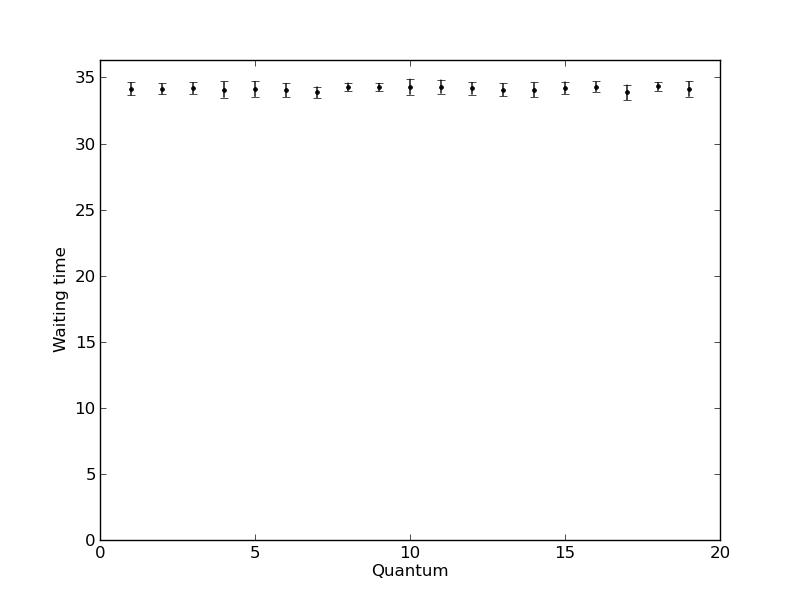
\includegraphics[width=8.75cm]{graficos/schedRR_celular/cores_3_wt.jpg}}
\hfill
\subfigure[]{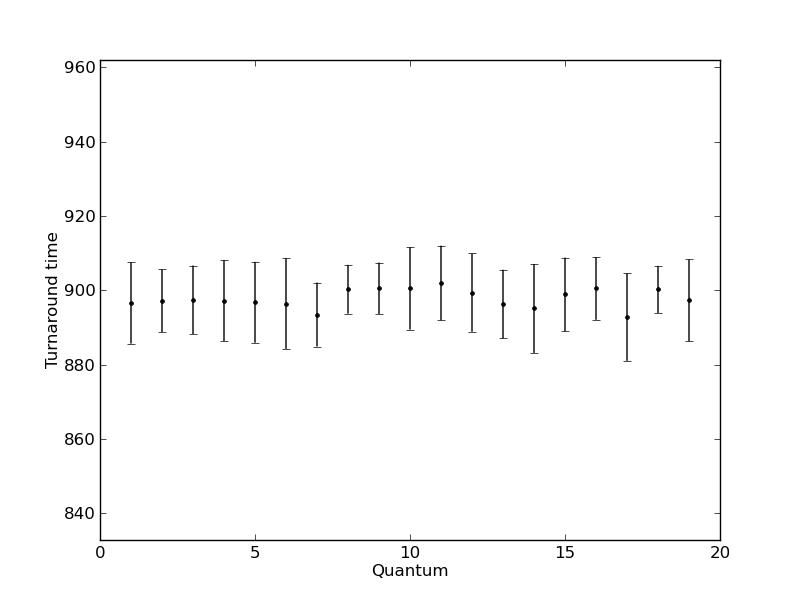
\includegraphics[width=8.75cm]{graficos/schedRR_celular/cores_3_ta.jpg}}
\hfill
\caption{Gráfico de Waiting time y turnaround time en función del quantum con 3 cores para lote de tareas $loteCelular$ en SchedRR}
\end{figure}

\begin{figure}[H]
\hfill
\subfigure[]{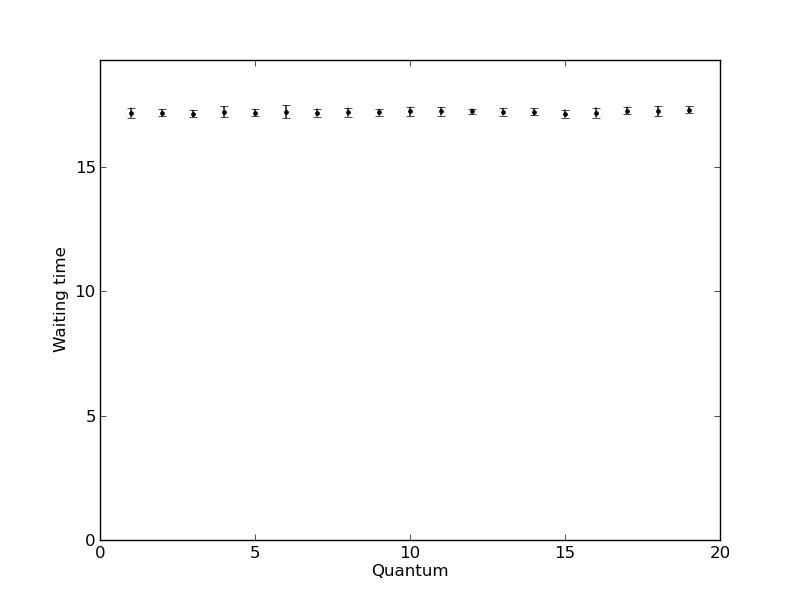
\includegraphics[width=8.75cm]{graficos/schedRR2_celular/cores_3_wt.jpg}}
\hfill
\subfigure[]{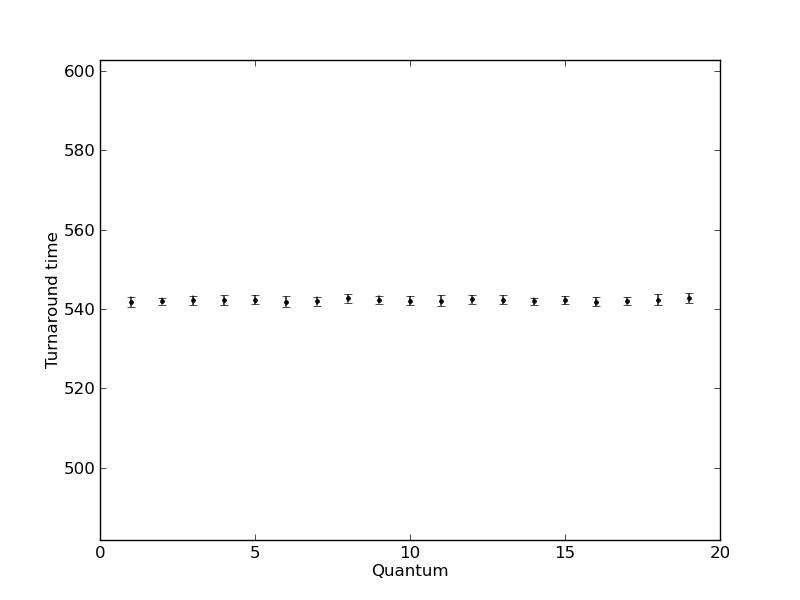
\includegraphics[width=8.75cm]{graficos/schedRR2_celular/cores_3_ta.jpg}}
\hfill
\caption{Gráfico de Waiting time y turnaround time en función del quantum con 3 cores para lote de tareas $loteCelular$ en SchedRR2}
\end{figure}

\begin{figure}[H]
\hfill
\subfigure[]{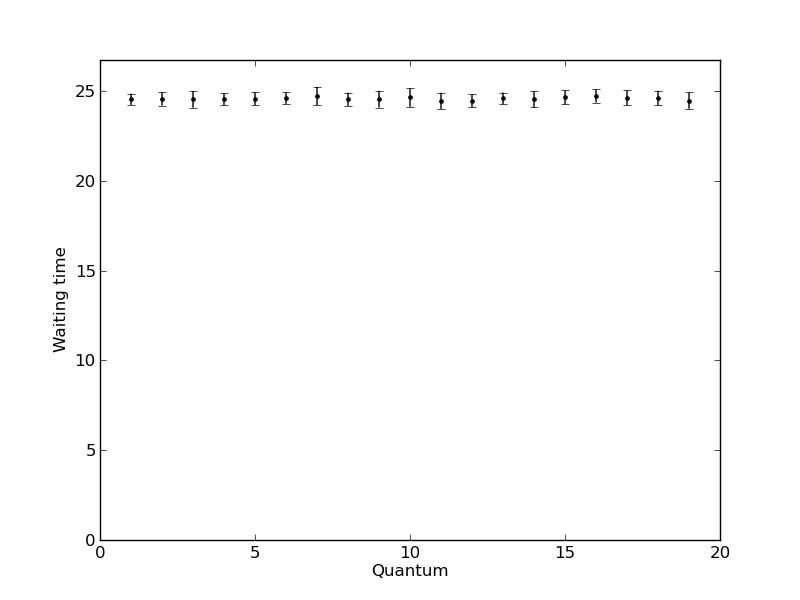
\includegraphics[width=8.75cm]{graficos/schedRR_celular/cores_4_wt.jpg}}
\hfill
\subfigure[]{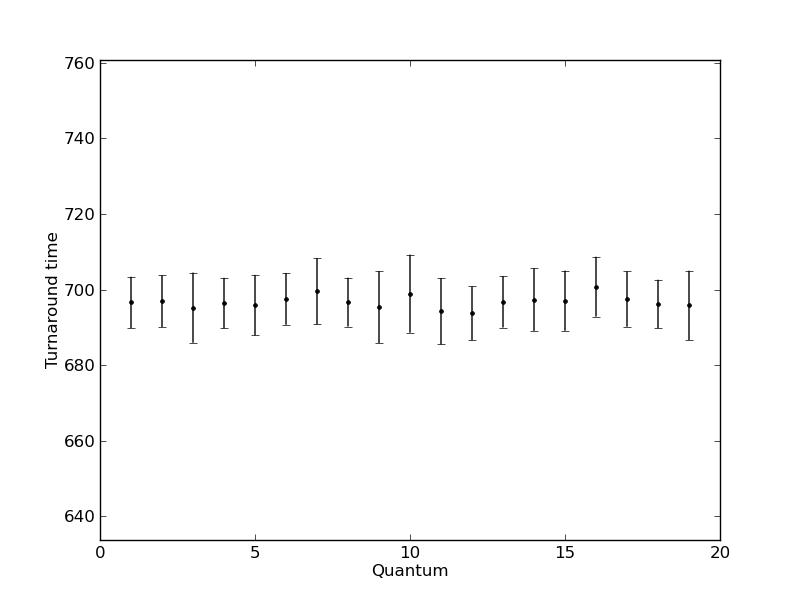
\includegraphics[width=8.75cm]{graficos/schedRR_celular/cores_4_ta.jpg}}
\hfill
\caption{Gráfico de Waiting time y turnaround time en función del quantum con 4 cores para lote de tareas $loteCelular$ en SchedRR}
\end{figure}

\begin{figure}[H]
\hfill
\subfigure[]{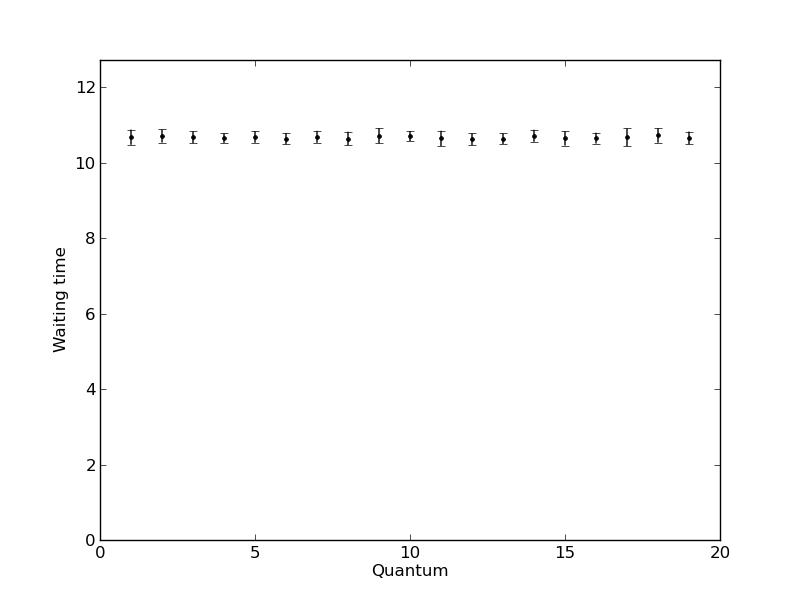
\includegraphics[width=8.75cm]{graficos/schedRR2_celular/cores_4_wt.jpg}}
\hfill
\subfigure[]{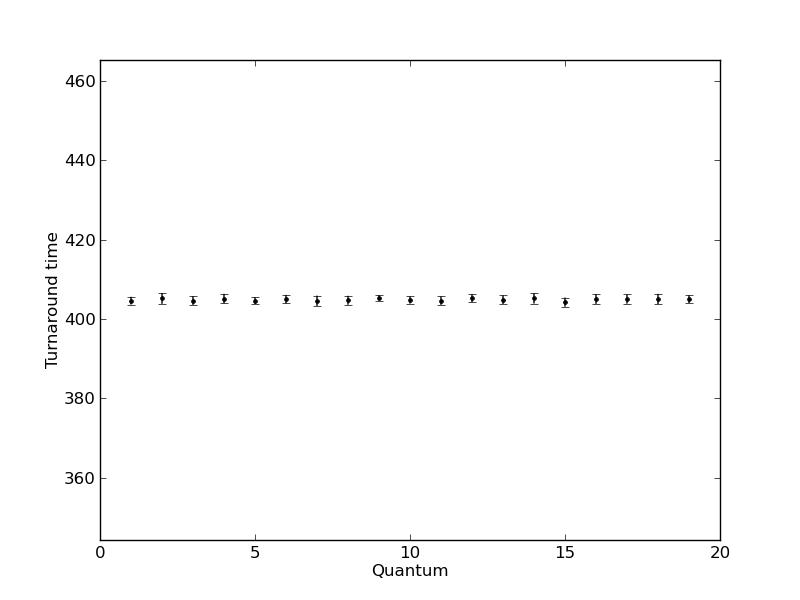
\includegraphics[width=8.75cm]{graficos/schedRR2_celular/cores_4_ta.jpg}}
\hfill
\caption{Gráfico de Waiting time y turnaround time en función del quantum con 4 cores para lote de tareas $loteCelular$ en SchedRR2}
\end{figure}

\begin{center}
    \begin{tabular}{ | l | l | l | l | l | p{5cm} |}
    \hline
    Cores & Wt RR & Wt RR2 & Ta RR & Ta RR2 \\ \hline
    2 & 48.96 & 30.25 & 1208.74 & 815.69 \\ \hline
    3 & 34.15 & 17.20 & 897.83 & 542.165 \\ \hline
    4 & 24.58 & 10.67 & 696.76 & 404.9 \\
	\hline
    \end{tabular}
\end{center}

Observando la tabla podemos concluir que el schedRR2 tiene un mejor wt y ta en promedio para un lote de tareas celular.

\subsubsection{Lote 3: uso intensivo de CPU}

\begin{figure}[H]
\hfill
\subfigure[]{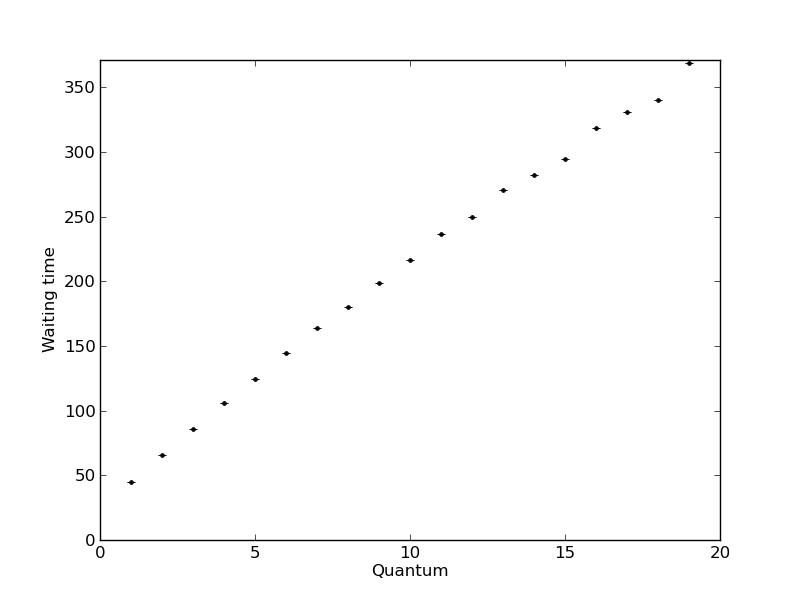
\includegraphics[width=8.75cm]{graficos/schedRR_cpu/cores_2_wt.jpg}}
\hfill
\subfigure[]{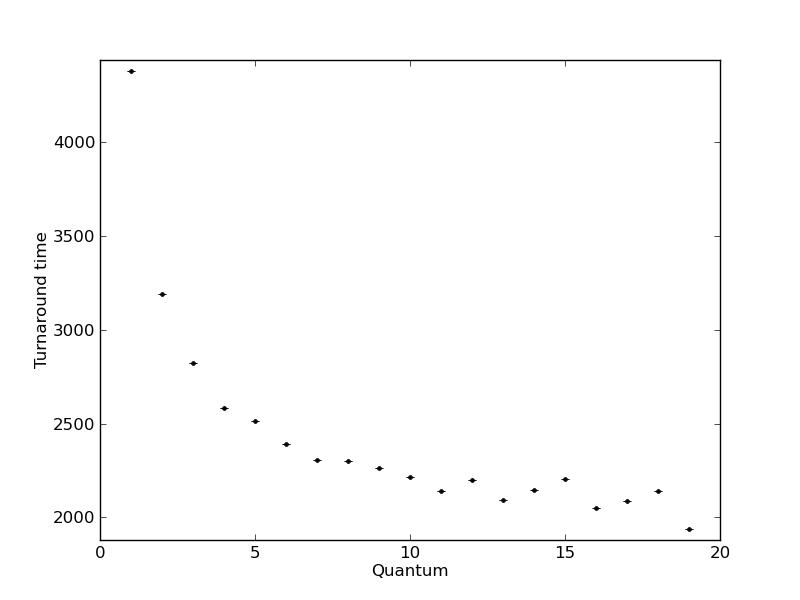
\includegraphics[width=8.75cm]{graficos/schedRR_cpu/cores_2_ta.jpg}}
\hfill
\caption{Gráfico de Waiting time y turnaround time en función del quantum con 2 cores para lote de tareas $loteCpu$ en SchedRR}
\end{figure}

\begin{figure}[H]
\hfill
\subfigure[]{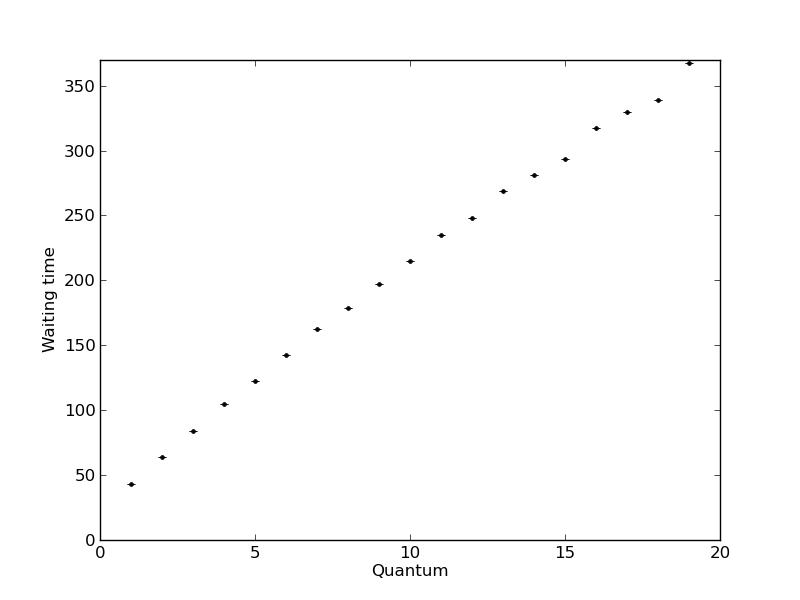
\includegraphics[width=8.75cm]{graficos/schedRR2_cpu/cores_2_wt.jpg}}
\hfill
\subfigure[]{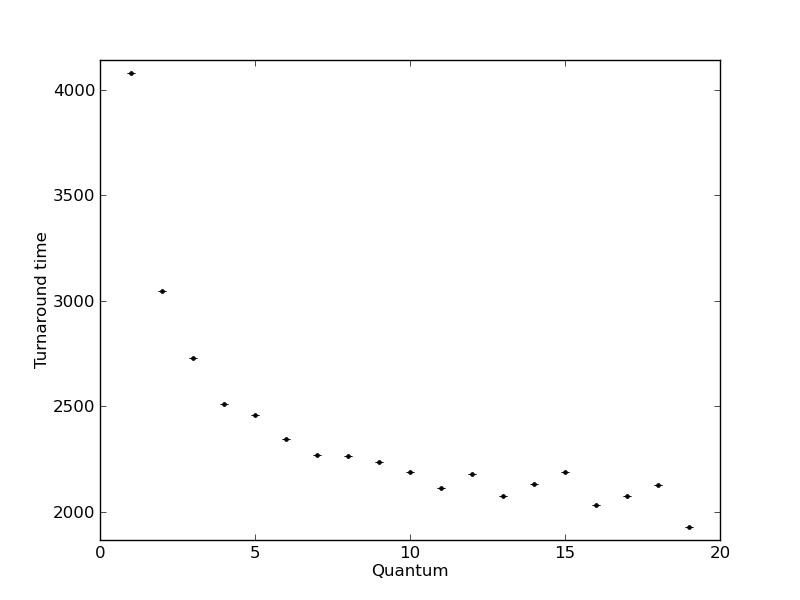
\includegraphics[width=8.75cm]{graficos/schedRR2_cpu/cores_2_ta.jpg}}
\hfill
\caption{Gráfico de Waiting time y turnaround time en función del quantum con 2 cores para lote de tareas $loteCpu$ en SchedRR2}
\end{figure}

\begin{figure}[H]
\hfill
\subfigure[]{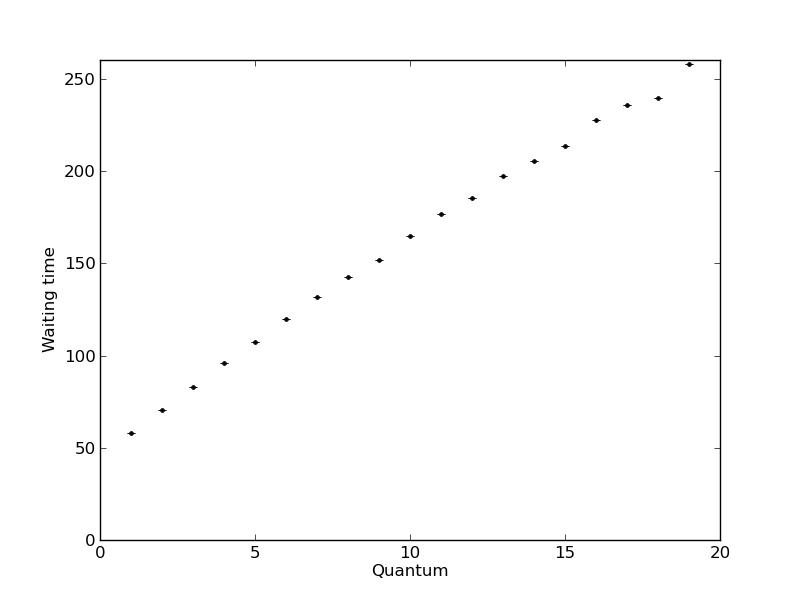
\includegraphics[width=8.75cm]{graficos/schedRR_cpu/cores_3_wt.jpg}}
\hfill
\subfigure[]{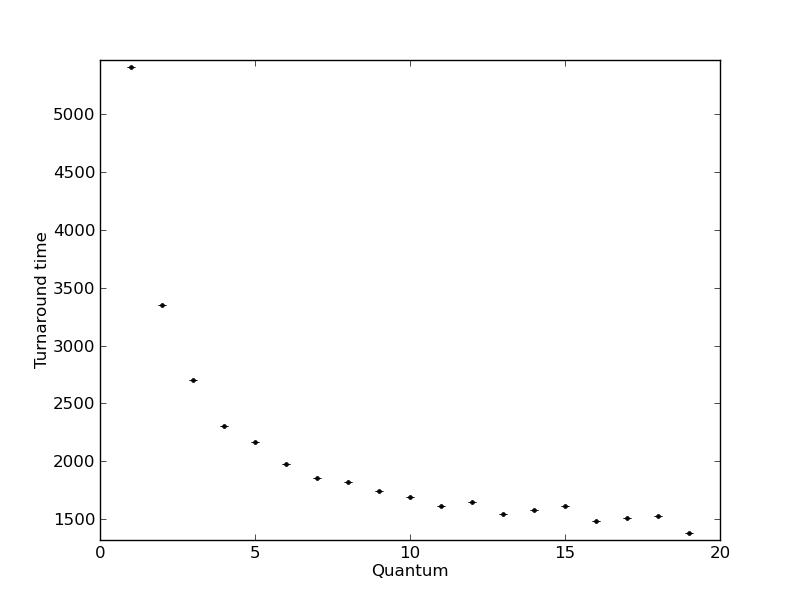
\includegraphics[width=8.75cm]{graficos/schedRR_cpu/cores_3_ta.jpg}}
\hfill
\caption{Gráfico de Waiting time y turnaround time en función del quantum con 3 cores para lote de tareas $loteCpu$ en SchedRR}
\end{figure}

\begin{figure}[H]
\hfill
\subfigure[]{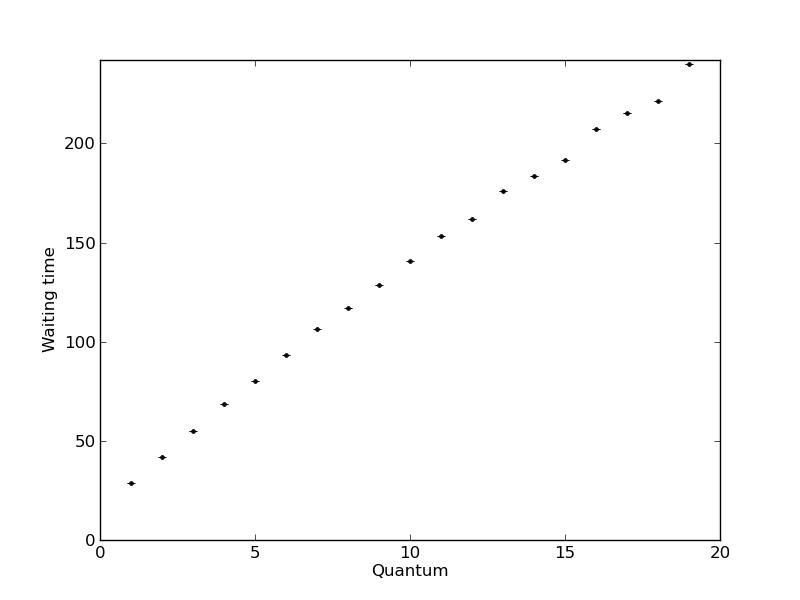
\includegraphics[width=8.75cm]{graficos/schedRR2_cpu/cores_3_wt.jpg}}
\hfill
\subfigure[]{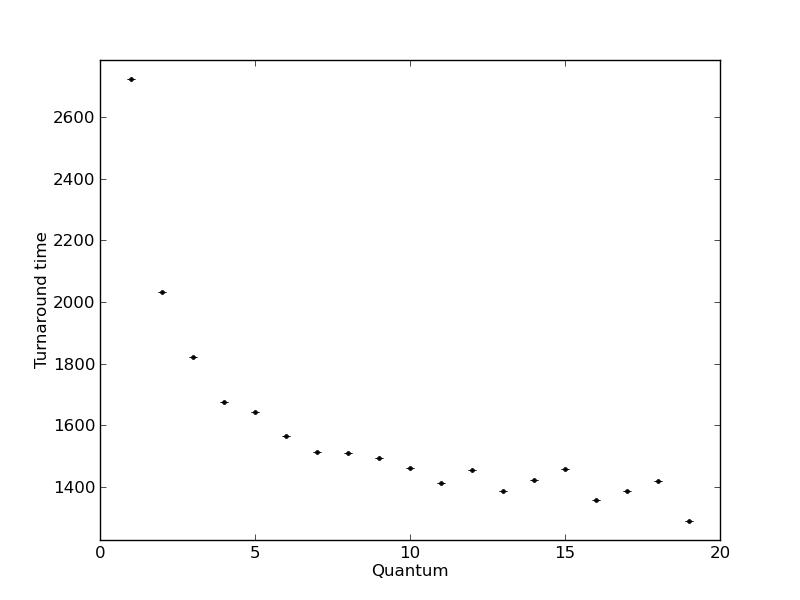
\includegraphics[width=8.75cm]{graficos/schedRR2_cpu/cores_3_ta.jpg}}
\hfill
\caption{Gráfico de Waiting time y turnaround time en función del quantum con 3 cores para lote de tareas $loteCpu$ en SchedRR2}
\end{figure}

\begin{figure}[H]
\hfill
\subfigure[]{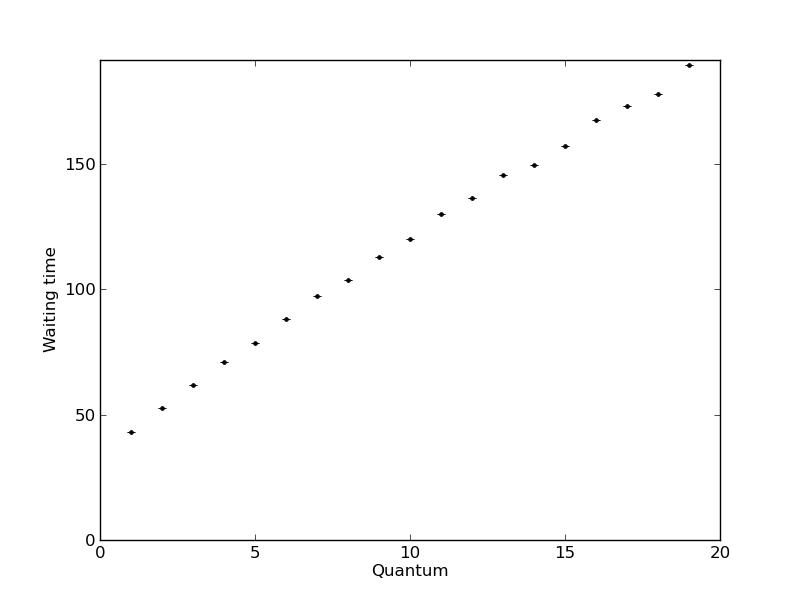
\includegraphics[width=8.75cm]{graficos/schedRR_cpu/cores_4_wt.jpg}}
\hfill
\subfigure[]{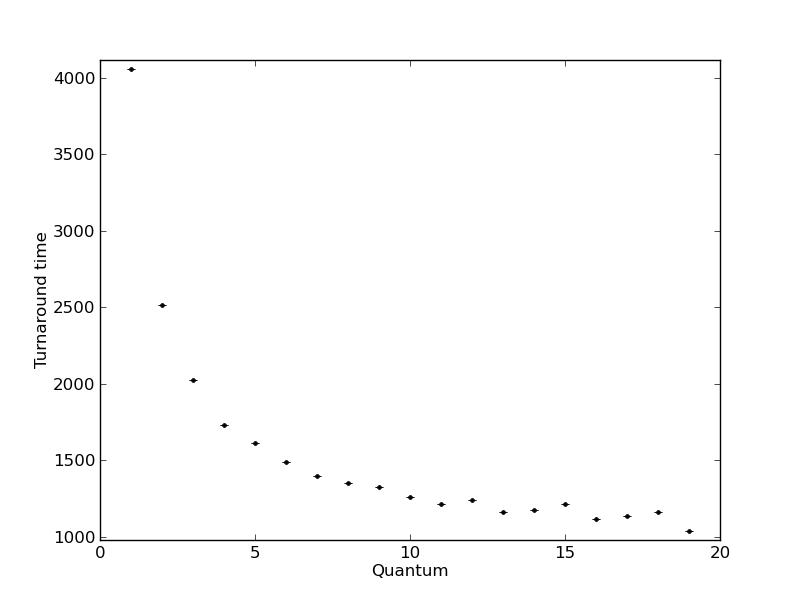
\includegraphics[width=8.75cm]{graficos/schedRR_cpu/cores_4_ta.jpg}}
\hfill
\caption{Gráfico de Waiting time y turnaround time en función del quantum con 4 cores para lote de tareas $loteCpu$ en SchedRR}
\end{figure}

\begin{figure}[H]
\hfill
\subfigure[]{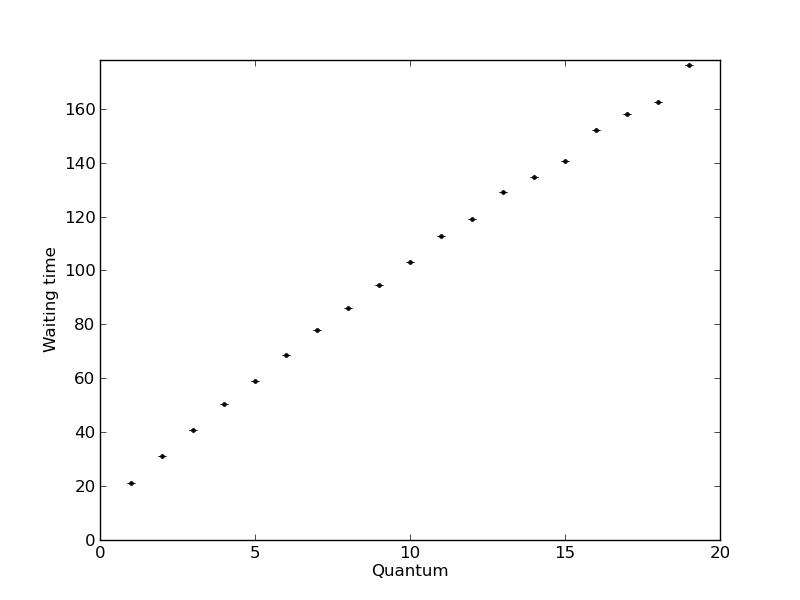
\includegraphics[width=8.75cm]{graficos/schedRR2_cpu/cores_4_wt.jpg}}
\hfill
\subfigure[]{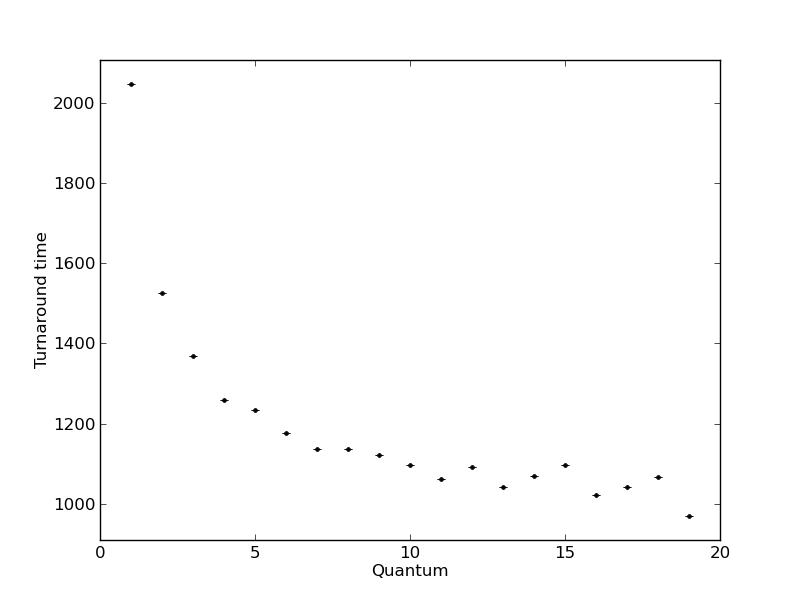
\includegraphics[width=8.75cm]{graficos/schedRR2_cpu/cores_4_ta.jpg}}
\hfill
\caption{Gráfico de Waiting time y turnaround time en función del quantum con 4 cores para lote de tareas $loteCpu$ en SchedRR2}
\end{figure}

\begin{center}
    \begin{tabular}{ | l | l | l | l | l | p{5cm} |}
    \hline
    Cores & Wt RR & Wt RR2 & Ta RR & Ta RR2 \\ \hline
    2 & 211.64 & 210.27 & 2419.82 & 2365.98 \\ \hline
    3 & 161.31 & 137.4 & 2049.82 & 1580.55 \\ \hline
    4 & 118.75 & 100.94 & 1537.24 & 1187.93 \\
	\hline
    \end{tabular}
\end{center}

Observando la tabla podemos concluir que el schedRR2 tiene un mejor wt y ta en promedio para un lote de tareas de uso intensivo de CPU.

En conclusión, podemos afirmar que el scheduler Round Robin que no permite migración de procesos entre núcleos (SchedRR2) funciona mejor que el SchedRR teniendo en cuenta las métricas de Turnaround time y Waiting time. Creemos que la diferencia de performance entre ambos schedulers radica en el hecho de que el SchedRR2 se ahorra los costos de migración cada vez que cambia de tarea.



\end{document}
